% Ensure that you compile using XeLaTeX !!! PDFTex has problems with some of the packages used
\documentclass[12pt]{article}
\setlength\parindent{0pt}

\usepackage{parskip}
\usepackage[margin=0.5in]{geometry}
\usepackage{fullpage}
\usepackage{moresize}
\usepackage{graphicx}
\usepackage{caption}
\usepackage{subcaption}
\usepackage{float}
\usepackage{xcolor}
\usepackage{soul}
\usepackage{fontspec}
\setmainfont{Doulos SIL}

\begin{document}

\begin{center}
\textbf{{\color{violet}{\HUGE Monday, 22 June 2020\\}}}

\textbf{{\color{violet}{\HUGE ALL EXAMS (with notes)\\}}}

\end{center}
\newpage

\begin{center}
\textbf{{\color{blue}{\HUGE START OF EXAM\\}}}

\textbf{{\color{blue}{\HUGE Student ID: 4066\\}}}

\textbf{{\color{blue}{\HUGE 2:20 - 2:40 PM\\}}}

\end{center}
\newpage

{\large Question 1}\\

Source: Day 9 Handout, Question 1\\

Explain why the concept of an alternation either is or is not useful for understanding this dataset.\\

\begin{figure}[H]
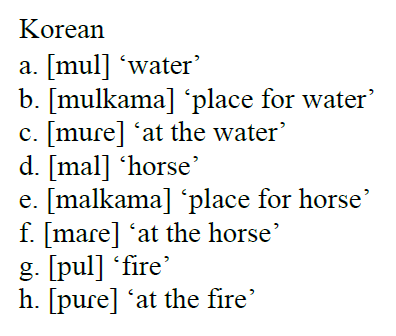
\includegraphics{../images/korean.png}
\end{figure}

~\\
INSTRUCTOR NOTES: is useful -- root morphemes alternate, so we can decide which sounds we need to analyze


\vfill
Excellent (3) ~~~ Good (2.2) ~~~ Fair (1.7) ~~~ Poor (0)
\newpage

{\large Question 2}\\

Source: Final Exam Dataset\\

Explain what the basic phonological analysis of this dataset is, and what the key pieces of evidence are.\\

\begin{figure}[H]
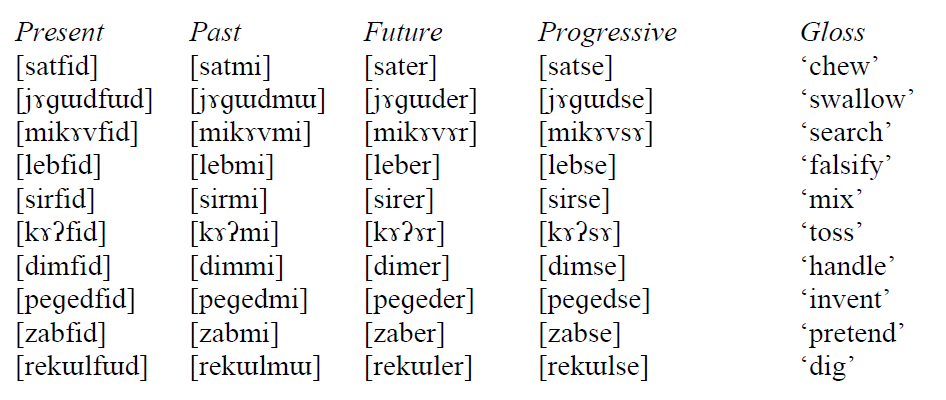
\includegraphics{../images/final_dataset.png}
\end{figure}

~\\
INSTRUCTOR NOTES: The basic analysis here is that vowels of the same height need to agree in terms of backness. We see this in suffix alternations: there are four alternating suffixes, each with a back and front variant, and two of them have high vowels while two of them have mid vowels. Whenever the suffix comes after a root containing a back vowel at the same height as the suffix, the suffix also contains a back vowel, but when the root contains either a front vowel or a back vowel at a different height, the suffix contains the front vowel. Thus, we posit the front versions as the URs of the suffixes, because they occur in the wider set of contexts, and write a rule of vowel backing that only applies when the target vowel follows a back context vowel of the same height.


\vfill
Excellent (3) ~~~ Good (2.2) ~~~ Fair (1.7) ~~~ Poor (0)
\newpage

{\large Question 3}\\

Source: Day 10 Discussion\\

Explain why the given feature's value varies across this set of sounds.\\

{[sonorant]}

alveolars


~\\
INSTRUCTOR NOTES: can have both sonorant and obstruent alveolars (e.g. [n] vs. [s])


\vfill
Excellent (3) ~~~ Good (2.2) ~~~ Fair (1.7) ~~~ Poor (0)
\newpage

{\large Question 4}\\

Source: Day 8 Handout, Question 7\\

Explain why each numbered, underlined statement is true or false. If it is false, explain one way that you could correct it.\\

We can look at the vertical location of the formants to determine something about the characteristics of individual speech sounds. For example, in the two spectrograms below, we can see that $^{22}$\ul{the first formant is higher in the spectrogram for sound 1 than it is for sound 2.} Because $^{23}$\ul{F1 is directly correlated with vowel height}, we know that $^{24}$\ul{the vowel pictured in sound 1 is a higher vowel than the one in sound 2}. For example, $^{25}$\ul{sound 1 might be an {[ɑ]} while sound 2 might be an {[i]}.}

\begin{figure}[H]
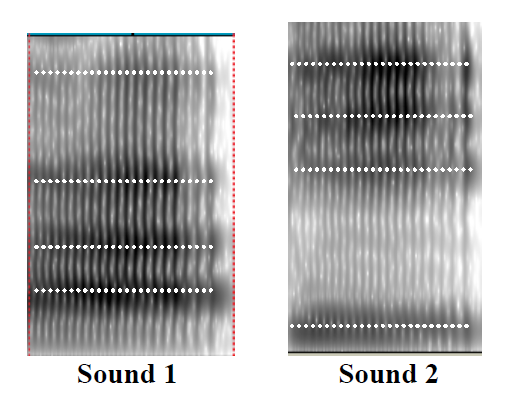
\includegraphics{../images/sound1a_sound2i.png}
\end{figure}

~\\
INSTRUCTOR NOTES: 22 - true. \\23 - false (F1 is inversely correlated with vowel height). \\24 - false (the vowel pictured in sound 1 is a lower vowel than the one in sound 2, or, the vowel pictured in sound 2 is a higher vowel than the one in sound 1).\\25 - true.


\vfill
Excellent (3) ~~~ Good (2.2) ~~~ Fair (1.7) ~~~ Poor (0)
\newpage

{\large Question 5}\\

Source: Quiz 10, Question 3\\

Section 4.2 of chapter 13 in the Peng textbook presented an autosegmental analysis of Mende tone distribution. Explain why the form shown below should NOT be the UR for any morpheme in Mende.\\

\begin{figure}[H]
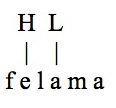
\includegraphics{../images/mende_junction_a.png}
\end{figure}

~\\
INSTRUCTOR NOTES: URs don't have pre-linked tones; the association lines are generated by rules (tone-mapping procedures)


\vfill
Excellent (3) ~~~ Good (2.2) ~~~ Fair (1.7) ~~~ Poor (0)
\newpage

{\large Question 6}\\

Source: Homework 5, Question 2\\

Explain why the insertion analysis is better than the deletion analysis for this dataset.\\

\begin{figure}[H]
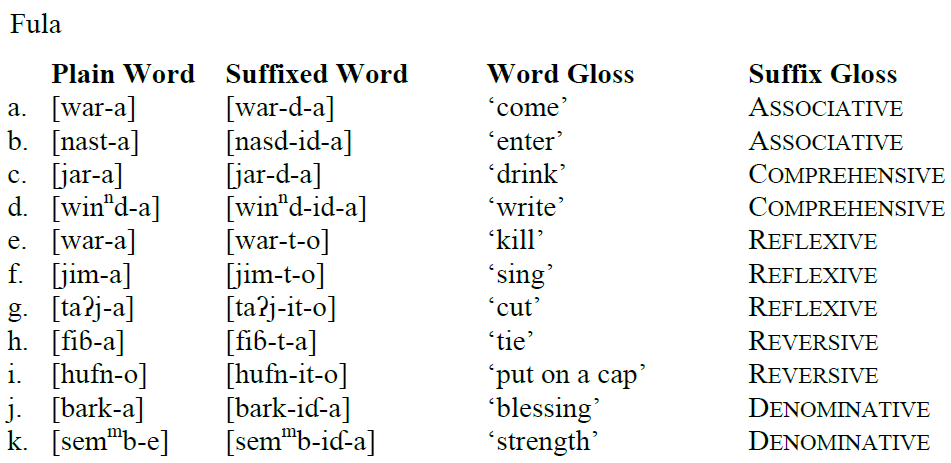
\includegraphics{../images/fula.png}
\end{figure}

~\\
INSTRUCTOR NOTES: If you have /VC/ as the underlying form of these suffixes, there’s no reason to delete the vowel, because you'd have perfect CV syllables throughout the word. But if you have /C/ as the underlying form, it’s clear that we occasionally need an extra vowel in order to allow syllabification to happen; otherwise, we’d end up with non-syllabifiable CCC sequences. That is, there’s a phonological motivation for the insertion rule, but no motivation for the deletion rule.


\vfill
Excellent (3) ~~~ Good (2.2) ~~~ Fair (1.7) ~~~ Poor (0)
\newpage

\begin{center}
\textbf{{\color{red}{\HUGE END OF EXAM}}}\\

\end{center}
\newpage

\begin{center}
\textbf{{\color{blue}{\HUGE START OF EXAM\\}}}

\textbf{{\color{blue}{\HUGE Student ID: 9246\\}}}

\textbf{{\color{blue}{\HUGE 2:40 - 3:00 PM\\}}}

\end{center}
\newpage

{\large Question 1}\\

Source: Day 11 Handout, Question 10\\

Explain why this structure either is or is not a correct application of the templatic-based approach to syllabification, using the provided template and assuming that syllabification proceeds from left to right.\\

\begin{figure}[H]
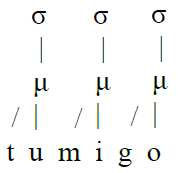
\includegraphics{../images/pengtemplate_tumigo_yes.png}
\end{figure}
\begin{figure}[H]
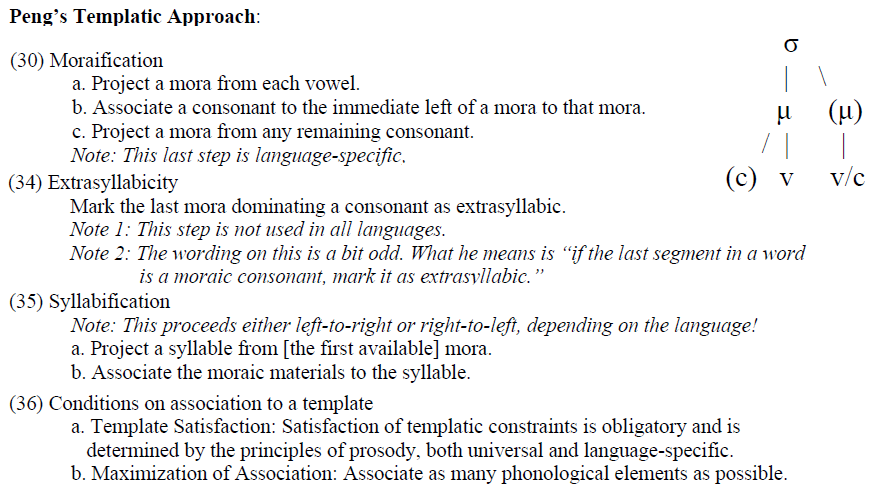
\includegraphics{../images/peng_template_withdiagram.png}
\end{figure}

~\\
INSTRUCTOR NOTES: yes; this is just all CV syllables


\vfill
Excellent (3) ~~~ Good (2.2) ~~~ Fair (1.7) ~~~ Poor (0)
\newpage

{\large Question 2}\\

Source: Final Exam Dataset\\

Give a good phonological description of the patterns in the dataset that should be analysed.\\

\begin{figure}[H]
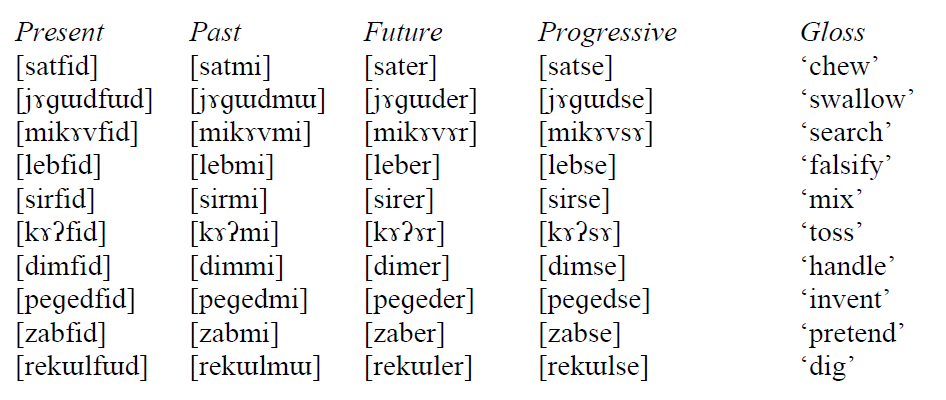
\includegraphics{../images/final_dataset.png}
\end{figure}

~\\
INSTRUCTOR NOTES: For each morpheme that alternates, there are two allomorphs, one with a front vowel and one with a back vowel. The allomorph with the back vowel occurs after another back vowel of the same height (e.g., [fɯd] in [jɤɡɯd-fɯd] ‘swallow, present’ or [sɤ] in [mikɤv-sɤ] ‘search, progressive’), regardless of any intervening consonants. The allomorph with the front vowel occurs elsewhere, including after a front vowel (e.g. [fid] in [sat-fid] ‘chew, present’ or [se] in [sat-se] ‘chew, progressive’) and after a back vowel of a different height (e.g. [fid] in [mikɤv-fid] ‘search, present’ or [se] in [jɤɡɯd-se] ‘swallow, progressive’). Again, these latter environments are regardless of any intervening consonants.


\vfill
Excellent (3) ~~~ Good (2.2) ~~~ Fair (1.7) ~~~ Poor (0)
\newpage

{\large Question 3}\\

Source: Day 8 Handout, Question 7\\

Explain why each numbered, underlined statement is true or false. If it is false, explain one way that you could correct it.\\

Sound is an invisible phenomenon. Sound can travel through any substance, $^1$\ul{such as a liquid, solid, or a gas.} $^2$\ul{It involves the transfer of the matter in that substance} from one place to another.\\\\Sound is a particular kind of wave known as $^3$\ul{a compression wave}. $^4$\ul{When the molecules are really close together, we say they are ``rarefied'' and when they are really far apart, we say they are ``compressed.''}


~\\
INSTRUCTOR NOTES: 1 - true.\\2 - false (it involves the transfer of energy... or anything about the matter itself not moving but only vibrating, etc). \\3 - true.\\4 - false (when the molecules are really close together, we say they are compressed and when the molecules are really far apart, we say they are rarefied).


\vfill
Excellent (3) ~~~ Good (2.2) ~~~ Fair (1.7) ~~~ Poor (0)
\newpage

{\large Question 4}\\

Source: Day 12 Handout, Question 7\\

What would be a good description of the alternation in this dataset?\\

\begin{figure}[H]
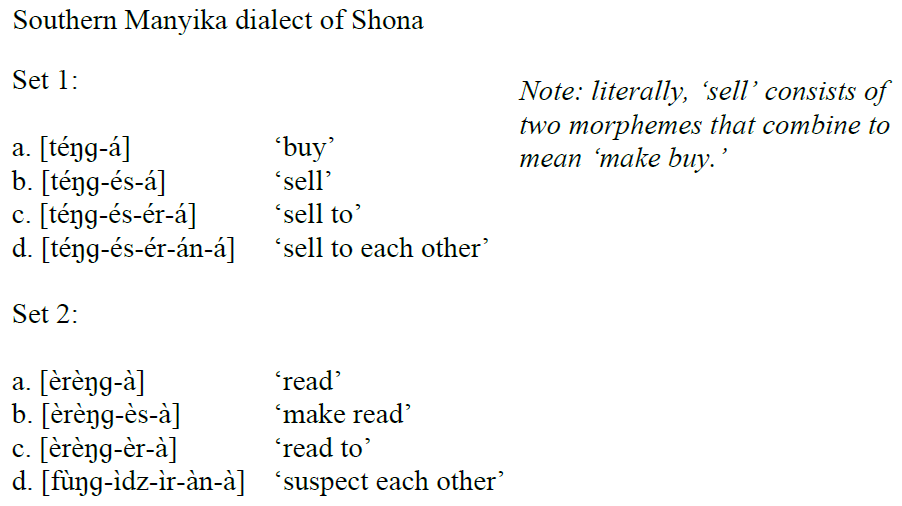
\includegraphics{../images/shona.png}
\end{figure}

~\\
INSTRUCTOR NOTES: The suffixes that alternate appear with a H tone after a H-toned root, and wtih a L tone after a L-toned root. For example, the causative suffix appears with a H tone, as [és], in [-téŋɡ-és-á] ‘sell,’ but with a L tone, as [ès], in [-èrèŋɡ-ès-à] ‘make read.’


\vfill
Excellent (3) ~~~ Good (2.2) ~~~ Fair (1.7) ~~~ Poor (0)
\newpage

{\large Question 5}\\

Source: Day 9 Handout, Question 5\\

Explain which morpheme(s) in this dataset alternate and how that helps you do a phonological analysis.\\

\begin{figure}[H]
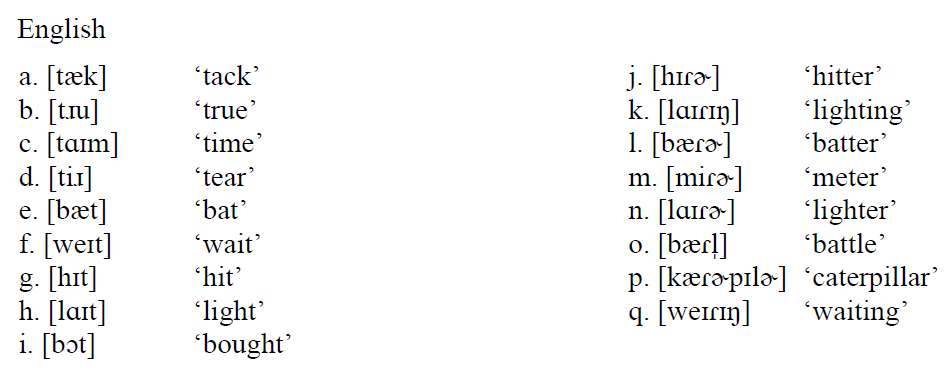
\includegraphics{../images/english_t_flap.png}
\end{figure}

~\\
INSTRUCTOR NOTES: some of the roots alternate (such as 'light'), so we know that we need to analyze the predictable occurrence of [t] vs. [flap]


\vfill
Excellent (3) ~~~ Good (2.2) ~~~ Fair (1.7) ~~~ Poor (0)
\newpage

{\large Question 6}\\

Source: Quiz 8, Question 6\\

Explain why this is an incorrect statement.\\

Nasal consonants are {[+continuant]}, because you can continue to make the sound for a long period of time (until you run out of breath).


~\\
INSTRUCTOR NOTES: nasals are [-cont], because air cannot escape through the mouth


\vfill
Excellent (3) ~~~ Good (2.2) ~~~ Fair (1.7) ~~~ Poor (0)
\newpage

\begin{center}
\textbf{{\color{red}{\HUGE END OF EXAM}}}\\

\end{center}
\newpage

\begin{center}
\textbf{{\color{blue}{\HUGE START OF EXAM\\}}}

\textbf{{\color{blue}{\HUGE Student ID: 4090\\}}}

\textbf{{\color{blue}{\HUGE 3:00 - 3:20 PM\\}}}

\end{center}
\newpage

{\large Question 1}\\

Source: Day 9 Handout, Question 1\\

Explain why the concept of an alternation either is or is not useful for understanding this dataset.\\

\begin{figure}[H]
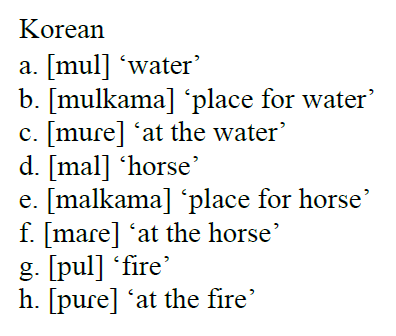
\includegraphics{../images/korean.png}
\end{figure}

~\\
INSTRUCTOR NOTES: is useful -- root morphemes alternate, so we can decide which sounds we need to analyze


\vfill
Excellent (3) ~~~ Good (2.2) ~~~ Fair (1.7) ~~~ Poor (0)
\newpage

{\large Question 2}\\

Source: Final Exam Dataset\\

Explain what the underlying representation of these morphemes would be and why.\\

`invent', `progressive'

\begin{figure}[H]
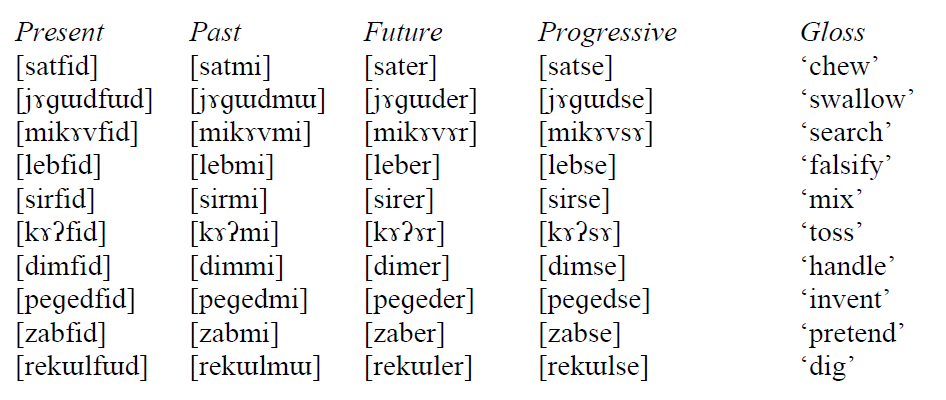
\includegraphics{../images/final_dataset.png}
\end{figure}

~\\
INSTRUCTOR NOTES: For any morpheme that doesn’t alternate, its UR should be the same as its SR.  For the morphemes that alternate, the back-vowel version occurs in the narrower set of contexts (after a back vowel of the same height), so should be the one that we write a rule for. The front-vowel version occurs in the wider / elsewhere set of contexts (after a front vowel and after a back vowel of a different height), so this should be the UR. So in this case, we have the non-alternating root morpheme ‘invent’ /peɡed/ and the alternating suffix morpheme 'progressive' /se/.


\vfill
Excellent (3) ~~~ Good (2.2) ~~~ Fair (1.7) ~~~ Poor (0)
\newpage

{\large Question 3}\\

Source: Day 11 Handout, Question 6\\

Explain why this structure either is or is not a correct application of the rule-based approach to syllabification, assuming that both the onset rule and the coda rule apply in this language, and the onset rule comes before the coda rule.\\

\begin{figure}[H]
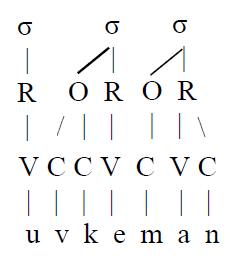
\includegraphics{../images/pengrules_uvkeman_yes.png}
\end{figure}
\begin{figure}[H]
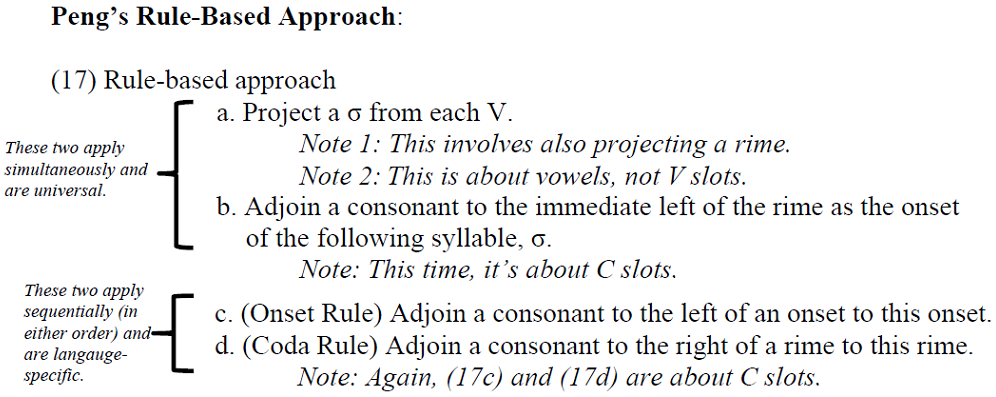
\includegraphics{../images/peng_rules.png}
\end{figure}

~\\
INSTRUCTOR NOTES: yes; the onset rule precedes the coda rule, which puts [v] into the onset (even though that violates sonority), but then we do get the [n] in coda position because it can't go into an onset, and the coda rule does apply


\vfill
Excellent (3) ~~~ Good (2.2) ~~~ Fair (1.7) ~~~ Poor (0)
\newpage

{\large Question 4}\\

Source: Day 8 Handout, Question 1\\

Explain what (if anything) the letter below represents on this waveform.\\

A

\begin{figure}[H]
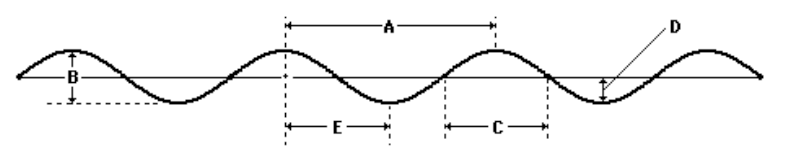
\includegraphics{../images/sinusoid.png}
\end{figure}

~\\
INSTRUCTOR NOTES: wavelength or period


\vfill
Excellent (3) ~~~ Good (2.2) ~~~ Fair (1.7) ~~~ Poor (0)
\newpage

{\large Question 5}\\

Source: Day 12 Handout, Question 5\\

Explain which of the three rules will apply to the form given below, and whether each of those rules would have an effect or not.\\

Peng’s Tone-Mapping Procedure for Mende: \begin{enumerate} \item L-to-R association: Associate the first tone to the first TBU, the second tone to the second TBU, and so on, until all tones or all TBUS are exhausted. \item Last-TBU Linking: Associate any remaining unlinked tones to the last TBU. \item Last-Tone Linking: Associate the last tone to any TBU without a tone. \end{enumerate}

\begin{figure}[H]
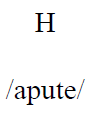
\includegraphics{../images/mendetone_b.png}
\end{figure}

~\\
INSTRUCTOR NOTES: L-to-R association applies and links the H tone to the first TBU [a]; last-TBU linking doesn't apply because there are no leftover tones; then last-tone linking does apply, and connects all of the leftover TBUs (in this case, [u] and [e]) to the final tone (in this case, H)


\vfill
Excellent (3) ~~~ Good (2.2) ~~~ Fair (1.7) ~~~ Poor (0)
\newpage

{\large Question 6}\\

Source: Day 10 Handout, Question 6 (Day 7 Handout, Question 7)\\

Explain how you should use phonological features to combine these rules.\\

/s/ → {[ʃ]} / \_\_ {[i]} \\/z/ → {[dʒ]} / \_\_ {[i]}

\begin{figure}[H]
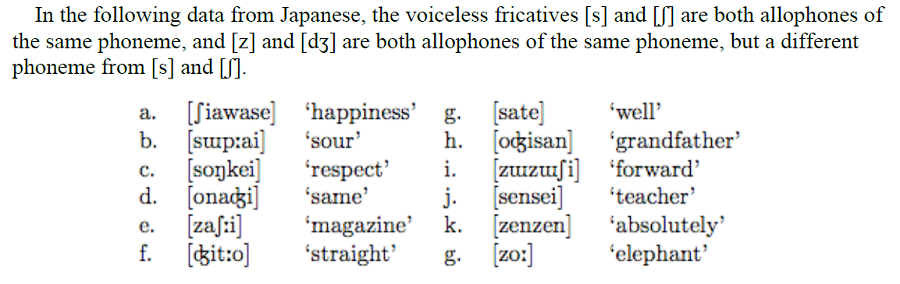
\includegraphics{../images/japanese.png}
\end{figure}

~\\
INSTRUCTOR NOTES: input should be alveolar fricatives, output should be just a change in place of articulation; context is still [i]; something like [CORONAL, +strid] --> [-ant, +dist] / \_\_ [i]; note that this won't directly account for why the voiced one becomes an affricate


\vfill
Excellent (3) ~~~ Good (2.2) ~~~ Fair (1.7) ~~~ Poor (0)
\newpage

\begin{center}
\textbf{{\color{red}{\HUGE END OF EXAM}}}\\

\end{center}
\newpage

\begin{center}
\textbf{{\color{blue}{\HUGE START OF EXAM\\}}}

\textbf{{\color{blue}{\HUGE Student ID: 1956\\}}}

\textbf{{\color{blue}{\HUGE 3:20 - 3:40 PM\\}}}

\end{center}
\newpage

{\large Question 1}\\

Source: Quiz 10, Question 3\\

Section 4.2 of chapter 13 in the Peng textbook presented an autosegmental analysis of Mende tone distribution. Explain why the form shown below should NOT be the UR for any morpheme in Mende.\\

\begin{figure}[H]
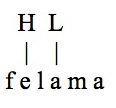
\includegraphics{../images/mende_junction_a.png}
\end{figure}

~\\
INSTRUCTOR NOTES: URs don't have pre-linked tones; the association lines are generated by rules (tone-mapping procedures)


\vfill
Excellent (3) ~~~ Good (2.2) ~~~ Fair (1.7) ~~~ Poor (0)
\newpage

{\large Question 2}\\

Source: Final Exam Dataset\\

Explain what the underlying representation of these morphemes would be and why.\\

`invent', `progressive'

\begin{figure}[H]
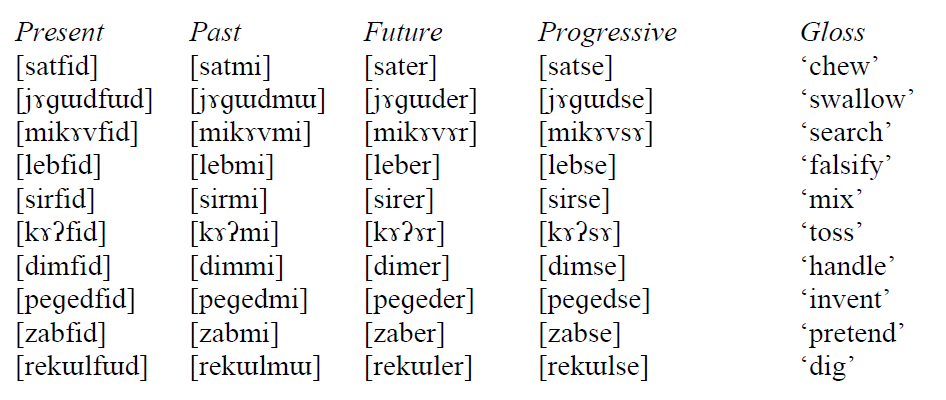
\includegraphics{../images/final_dataset.png}
\end{figure}

~\\
INSTRUCTOR NOTES: For any morpheme that doesn’t alternate, its UR should be the same as its SR.  For the morphemes that alternate, the back-vowel version occurs in the narrower set of contexts (after a back vowel of the same height), so should be the one that we write a rule for. The front-vowel version occurs in the wider / elsewhere set of contexts (after a front vowel and after a back vowel of a different height), so this should be the UR. So in this case, we have the non-alternating root morpheme ‘invent’ /peɡed/ and the alternating suffix morpheme 'progressive' /se/.


\vfill
Excellent (3) ~~~ Good (2.2) ~~~ Fair (1.7) ~~~ Poor (0)
\newpage

{\large Question 3}\\

Source: Day 8 Handout, Question 7\\

Explain why each numbered, underlined statement is true or false. If it is false, explain one way that you could correct it.\\

$^{10}$\ul{Frequency is inversely related to pitch: high frequencies correspond to low pitches, and low frequencies correspond to high pitches.} Finally, there is the amplitude of the wave. $^{11}$\ul{The amplitude tells you how much pressure the molecules are under at any particular time.} $^{12}$\ul{The auditory correlate of amplitude is intensity}; this is a measure of perceived pressure.\\\\$^{13}$\ul{In speech, air is set in vibrating motion by the lungs, so the lungs} are the source of most speech sounds.


~\\
INSTRUCTOR NOTES: 10 - false (frequency is directly related to pitch: high frequencies correspond to high pitches, and low frequencies correspond to low pitches).\\11 - true.\\12 - false (the auditory correlate of amplitude and intensity is loudness/volume, or, a related acoustic measure to amplitude is intensity).\\13 - false (air is set in vibrating motion by the vocal folds).


\vfill
Excellent (3) ~~~ Good (2.2) ~~~ Fair (1.7) ~~~ Poor (0)
\newpage

{\large Question 4}\\

Source: Day 11 Handout, Question 14\\

How does syllabification play a role in the analysis of the phonological relationship between tense and lax high vowels in Quebec French?\\

\begin{figure}[H]
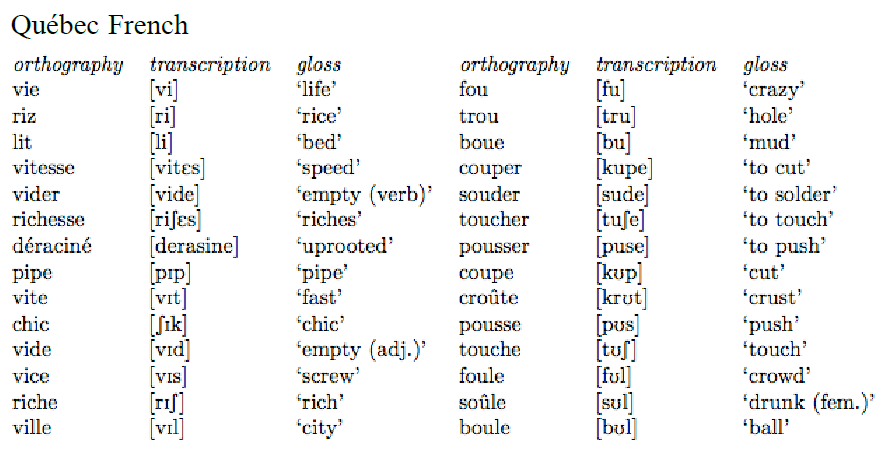
\includegraphics{../images/quebecfrench.png}
\end{figure}

~\\
INSTRUCTOR NOTES: here, syllabification must precede the rest of the analysis; the tense vowels ([i] and [u]) occur in open syllables, while the lax vowels occur in closed syllables -- so e.g. we might have a rule of vowel laxing that says [+high, +syll] --> [-tense] / \_\_ C., with a period to specifically mark the syllable boundary in the context of the rule


\vfill
Excellent (3) ~~~ Good (2.2) ~~~ Fair (1.7) ~~~ Poor (0)
\newpage

{\large Question 5}\\

Source: Day 9 Handout, Question 5\\

Explain which morpheme(s) in this dataset alternate and how that helps you do a phonological analysis.\\

\begin{figure}[H]
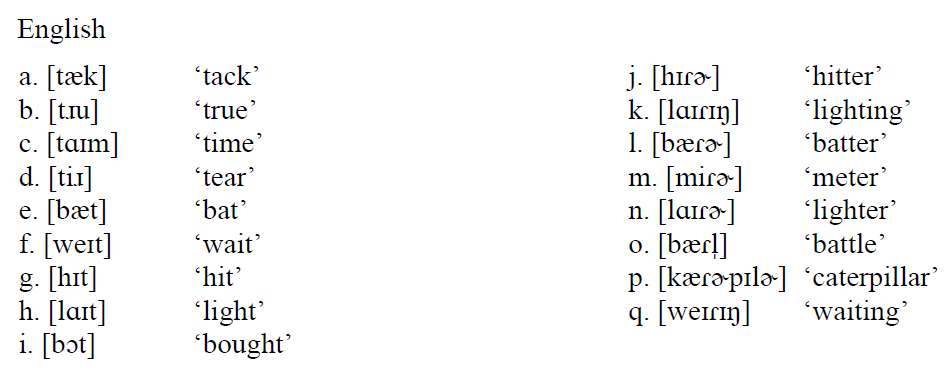
\includegraphics{../images/english_t_flap.png}
\end{figure}

~\\
INSTRUCTOR NOTES: some of the roots alternate (such as 'light'), so we know that we need to analyze the predictable occurrence of [t] vs. [flap]


\vfill
Excellent (3) ~~~ Good (2.2) ~~~ Fair (1.7) ~~~ Poor (0)
\newpage

{\large Question 6}\\

Source: Day 10 Discussion\\

Explain why the given feature's value varies across this set of sounds.\\

{[voice]}

glottalized obstruents


~\\
INSTRUCTOR NOTES: includes both voiced and voiceless glottalized obstruents -- obs. can themselves be voiced or voiceless


\vfill
Excellent (3) ~~~ Good (2.2) ~~~ Fair (1.7) ~~~ Poor (0)
\newpage

\begin{center}
\textbf{{\color{red}{\HUGE END OF EXAM}}}\\

\end{center}
\newpage

\begin{center}
\textbf{{\color{blue}{\HUGE START OF EXAM\\}}}

\textbf{{\color{blue}{\HUGE Student ID: 3737\\}}}

\textbf{{\color{blue}{\HUGE 3:40 - 4:00 PM\\}}}

\end{center}
\newpage

{\large Question 1}\\

Source: Day 11 Handout, Question 5\\

Explain why this template either does or does not allow syllables of this type to occur.\\

CCV

\begin{figure}[H]
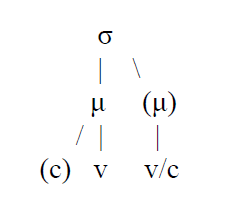
\includegraphics{../images/ponapean_syllabletemplate.png}
\end{figure}

~\\
INSTRUCTOR NOTES: not allowed


\vfill
Excellent (3) ~~~ Good (2.2) ~~~ Fair (1.7) ~~~ Poor (0)
\newpage

{\large Question 2}\\

Source: Final Exam Dataset\\

Explain what the underlying representation of these morphemes would be and why.\\

`invent', `progressive'

\begin{figure}[H]
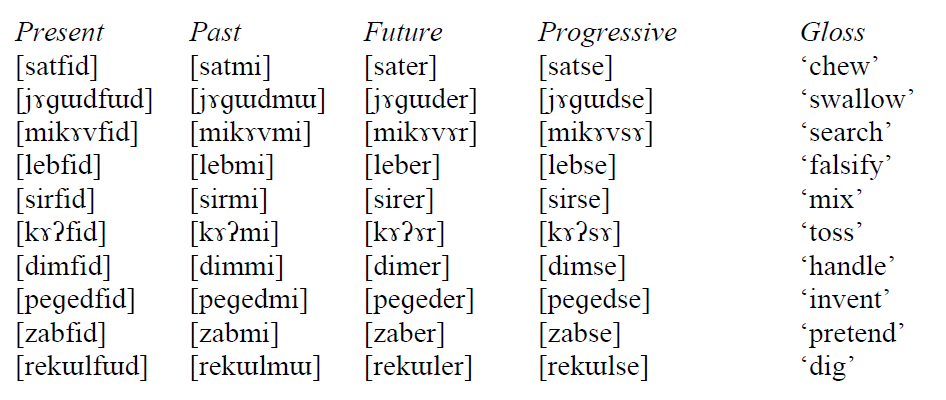
\includegraphics{../images/final_dataset.png}
\end{figure}

~\\
INSTRUCTOR NOTES: For any morpheme that doesn’t alternate, its UR should be the same as its SR.  For the morphemes that alternate, the back-vowel version occurs in the narrower set of contexts (after a back vowel of the same height), so should be the one that we write a rule for. The front-vowel version occurs in the wider / elsewhere set of contexts (after a front vowel and after a back vowel of a different height), so this should be the UR. So in this case, we have the non-alternating root morpheme ‘invent’ /peɡed/ and the alternating suffix morpheme 'progressive' /se/.


\vfill
Excellent (3) ~~~ Good (2.2) ~~~ Fair (1.7) ~~~ Poor (0)
\newpage

{\large Question 3}\\

Source: Day 12 Handout, Question 5\\

Explain which of the three rules will apply to the form given below, and whether each of those rules would have an effect or not.\\

Peng’s Tone-Mapping Procedure for Mende: \begin{enumerate} \item L-to-R association: Associate the first tone to the first TBU, the second tone to the second TBU, and so on, until all tones or all TBUS are exhausted. \item Last-TBU Linking: Associate any remaining unlinked tones to the last TBU. \item Last-Tone Linking: Associate the last tone to any TBU without a tone. \end{enumerate}

\begin{figure}[H]
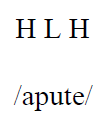
\includegraphics{../images/mendetone_a.png}
\end{figure}

~\\
INSTRUCTOR NOTES: L-to-R association is the only one that applies; it links up each of the three tones to a TBU, and then the other rules have nothing to do, because their context isn't met (there are no leftover tones or TBUs)


\vfill
Excellent (3) ~~~ Good (2.2) ~~~ Fair (1.7) ~~~ Poor (0)
\newpage

{\large Question 4}\\

Source: Day 8 Handout, Question 3\\

Explain what you see in the spectrogram that tells you about the properties of the sounds in the pictured word.\\

\begin{figure}[H]
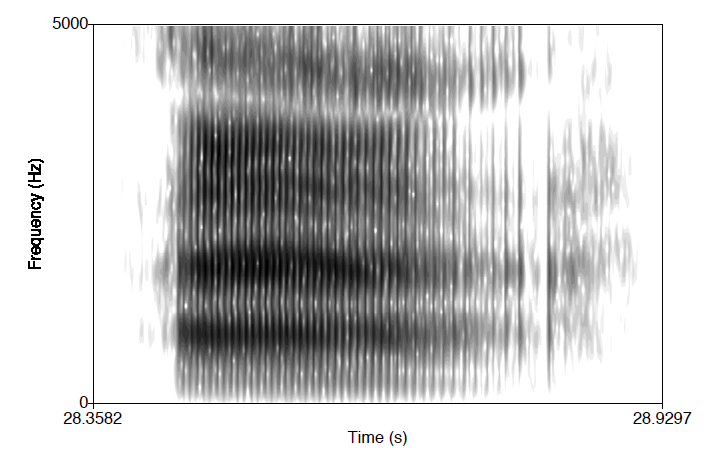
\includegraphics{../images/spectrogram_aaah.png}
\end{figure}

~\\
INSTRUCTOR NOTES: aaah: just a vowel; formants are very steady; F1 and F2 are pretty close to each other; F1 somewhat high and F2 somewhat low


\vfill
Excellent (3) ~~~ Good (2.2) ~~~ Fair (1.7) ~~~ Poor (0)
\newpage

{\large Question 5}\\

Source: Day 10 Discussion\\

Explain why the given feature's value varies across this set of sounds.\\

{[voice]}

glottalized obstruents


~\\
INSTRUCTOR NOTES: includes both voiced and voiceless glottalized obstruents -- obs. can themselves be voiced or voiceless


\vfill
Excellent (3) ~~~ Good (2.2) ~~~ Fair (1.7) ~~~ Poor (0)
\newpage

{\large Question 6}\\

Source: Day 9 Handout, Question 3\\

Explain which morpheme(s) in this dataset alternate and how that helps you do a phonological analysis.\\

\begin{figure}[H]
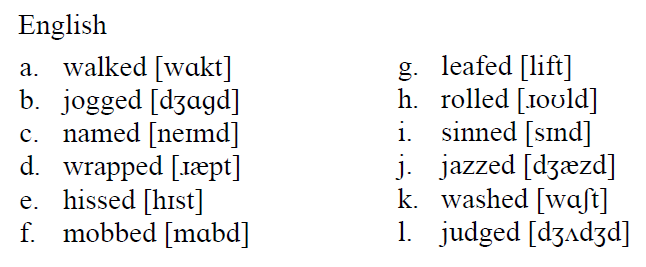
\includegraphics{../images/english_past.png}
\end{figure}

~\\
INSTRUCTOR NOTES: the past tense morpheme alternates, so we know we need to analyze the predictable occurrence of [t] vs. [d]


\vfill
Excellent (3) ~~~ Good (2.2) ~~~ Fair (1.7) ~~~ Poor (0)
\newpage

\begin{center}
\textbf{{\color{red}{\HUGE END OF EXAM}}}\\

\end{center}
\newpage

\begin{center}
\textbf{{\color{blue}{\HUGE START OF EXAM\\}}}

\textbf{{\color{blue}{\HUGE Student ID: 4465\\}}}

\textbf{{\color{blue}{\HUGE 4:00 - 4:20 PM\\}}}

\end{center}
\newpage

{\large Question 1}\\

Source: Day 11 Handout, Question 12\\

Explain why what you’re analyzing in the following dataset either is or is not an alternation.\\

\begin{figure}[H]
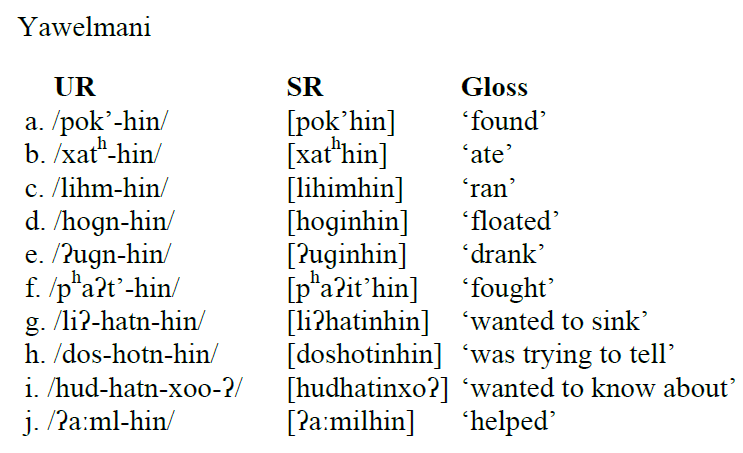
\includegraphics{../images/yawelmani.png}
\end{figure}

~\\
INSTRUCTOR NOTES: it's not an alternation -- we don't have multiple *surface* forms of the same morpheme; the different forms are the UR and the SR, and so they are not predictable from phonological context (the SR is derived from the UR by rule)


\vfill
Excellent (3) ~~~ Good (2.2) ~~~ Fair (1.7) ~~~ Poor (0)
\newpage

{\large Question 2}\\

Source: Final Exam Dataset\\

Explain what the underlying representation of these morphemes would be and why.\\

`search', `present'

\begin{figure}[H]
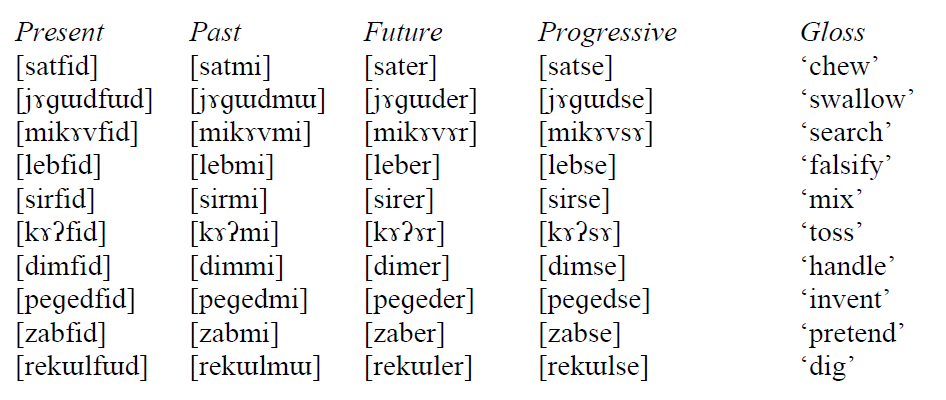
\includegraphics{../images/final_dataset.png}
\end{figure}

~\\
INSTRUCTOR NOTES: For any morpheme that doesn’t alternate, its UR should be the same as its SR.  For the morphemes that alternate, the back-vowel version occurs in the narrower set of contexts (after a back vowel of the same height), so should be the one that we write a rule for. The front-vowel version occurs in the wider / elsewhere set of contexts (after a front vowel and after a back vowel of a different height), so this should be the UR. So in this case, we have the non-alternating root morpheme ‘search’ /mikɤv/ and the alternating suffix morpheme 'present' /fid/.


\vfill
Excellent (3) ~~~ Good (2.2) ~~~ Fair (1.7) ~~~ Poor (0)
\newpage

{\large Question 3}\\

Source: Day 10 Handout, Question 6 (Homework 4, Question 2)\\

Explain how you should use phonological features in this rule. Which parts of the rule should include features, and what features might they be? You don't have to give an exact set of features, but what kinds of features would be involved?\\

/n/ → ∅ / {[m]} \_\_ \#

\begin{figure}[H]
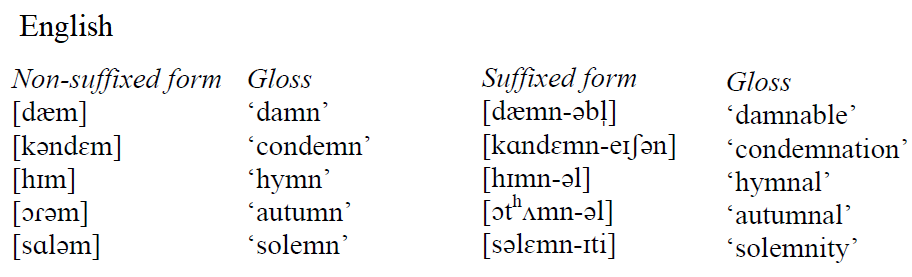
\includegraphics{../images/english_stemalternations.png}
\end{figure}

~\\
INSTRUCTOR NOTES: you really can't use features for any of this, because it's all individual segments


\vfill
Excellent (3) ~~~ Good (2.2) ~~~ Fair (1.7) ~~~ Poor (0)
\newpage

{\large Question 4}\\

Source: Day 11 Handout, Question 10\\

Explain why this structure either is or is not a correct application of the templatic-based approach to syllabification, using the provided template and assuming that syllabification proceeds from left to right.\\

\begin{figure}[H]
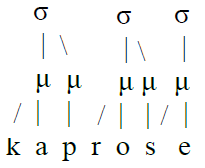
\includegraphics{../images/pengtemplate_kaprosse_yes.png}
\end{figure}
\begin{figure}[H]
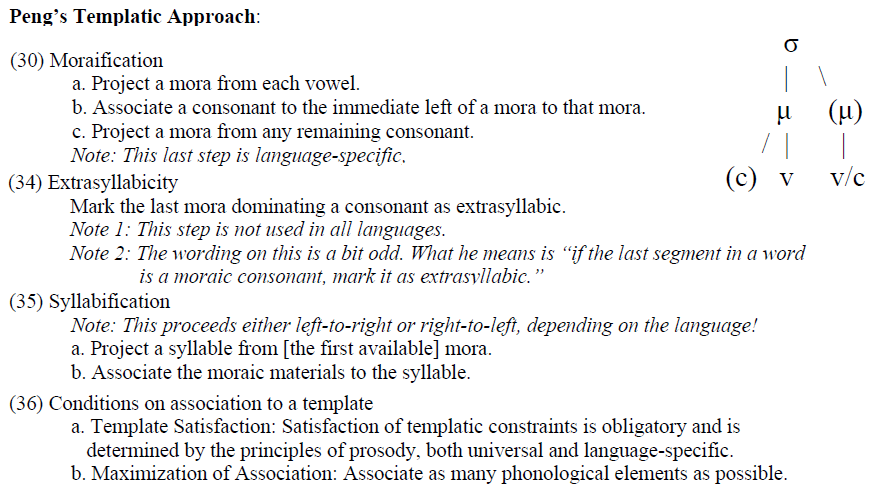
\includegraphics{../images/peng_template_withdiagram.png}
\end{figure}

~\\
INSTRUCTOR NOTES: yes; all syllables allowed by template, and this is what you get going L to R


\vfill
Excellent (3) ~~~ Good (2.2) ~~~ Fair (1.7) ~~~ Poor (0)
\newpage

{\large Question 5}\\

Source: Day 12 Handout, Question 5\\

Explain which of the three rules will apply to the form given below, and whether each of those rules would have an effect or not.\\

Peng’s Tone-Mapping Procedure for Mende: \begin{enumerate} \item L-to-R association: Associate the first tone to the first TBU, the second tone to the second TBU, and so on, until all tones or all TBUS are exhausted. \item Last-TBU Linking: Associate any remaining unlinked tones to the last TBU. \item Last-Tone Linking: Associate the last tone to any TBU without a tone. \end{enumerate}

\begin{figure}[H]
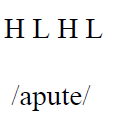
\includegraphics{../images/mendetone_d.png}
\end{figure}

~\\
INSTRUCTOR NOTES: L-to-R association applies, and links the first three tones (H L H) to the first three TBUs ([a], [u], [e]). Then last-TBU linking applies and links the leftover L tone to the last TBU ([e]). Last-tone linking will not apply because there are no leftover TBUs.


\vfill
Excellent (3) ~~~ Good (2.2) ~~~ Fair (1.7) ~~~ Poor (0)
\newpage

{\large Question 6}\\

Source: Day 8 Handout, Question 1\\

Explain what (if anything) the letter below represents on this waveform.\\

D

\begin{figure}[H]
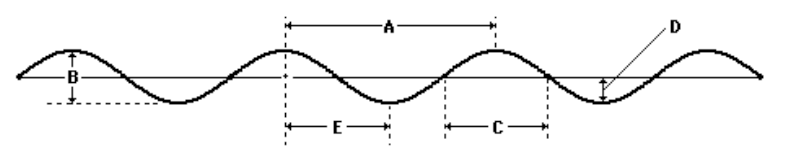
\includegraphics{../images/sinusoid.png}
\end{figure}

~\\
INSTRUCTOR NOTES: amplitude


\vfill
Excellent (3) ~~~ Good (2.2) ~~~ Fair (1.7) ~~~ Poor (0)
\newpage

\begin{center}
\textbf{{\color{red}{\HUGE END OF EXAM}}}\\

\end{center}
\newpage

\begin{center}
\textbf{{\color{blue}{\HUGE START OF EXAM\\}}}

\textbf{{\color{blue}{\HUGE Student ID: 9376\\}}}

\textbf{{\color{blue}{\HUGE 4:20 - 4:40 PM\\}}}

\end{center}
\newpage

{\large Question 1}\\

Source: Day 8 Handout, Question 1\\

Explain what (if anything) the letter below represents on this waveform.\\

C

\begin{figure}[H]
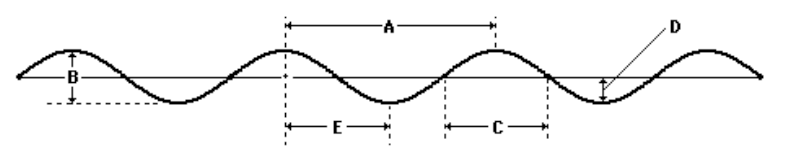
\includegraphics{../images/sinusoid.png}
\end{figure}

~\\
INSTRUCTOR NOTES: nothing (half wavelength or half period)


\vfill
Excellent (3) ~~~ Good (2.2) ~~~ Fair (1.7) ~~~ Poor (0)
\newpage

{\large Question 2}\\

Source: Day 12 Handout, Question 5\\

Explain which of the three rules will apply to the form given below, and whether each of those rules would have an effect or not.\\

Peng’s Tone-Mapping Procedure for Mende: \begin{enumerate} \item L-to-R association: Associate the first tone to the first TBU, the second tone to the second TBU, and so on, until all tones or all TBUS are exhausted. \item Last-TBU Linking: Associate any remaining unlinked tones to the last TBU. \item Last-Tone Linking: Associate the last tone to any TBU without a tone. \end{enumerate}

\begin{figure}[H]
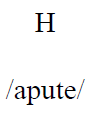
\includegraphics{../images/mendetone_b.png}
\end{figure}

~\\
INSTRUCTOR NOTES: L-to-R association applies and links the H tone to the first TBU [a]; last-TBU linking doesn't apply because there are no leftover tones; then last-tone linking does apply, and connects all of the leftover TBUs (in this case, [u] and [e]) to the final tone (in this case, H)


\vfill
Excellent (3) ~~~ Good (2.2) ~~~ Fair (1.7) ~~~ Poor (0)
\newpage

{\large Question 3}\\

Source: Final Exam Dataset\\

Explain what the underlying representation of these morphemes would be and why.\\

`search', `present'

\begin{figure}[H]
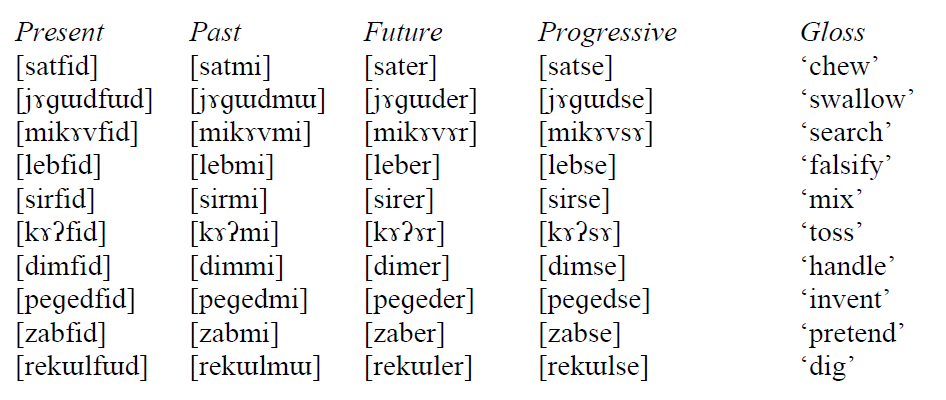
\includegraphics{../images/final_dataset.png}
\end{figure}

~\\
INSTRUCTOR NOTES: For any morpheme that doesn’t alternate, its UR should be the same as its SR.  For the morphemes that alternate, the back-vowel version occurs in the narrower set of contexts (after a back vowel of the same height), so should be the one that we write a rule for. The front-vowel version occurs in the wider / elsewhere set of contexts (after a front vowel and after a back vowel of a different height), so this should be the UR. So in this case, we have the non-alternating root morpheme ‘search’ /mikɤv/ and the alternating suffix morpheme 'present' /fid/.


\vfill
Excellent (3) ~~~ Good (2.2) ~~~ Fair (1.7) ~~~ Poor (0)
\newpage

{\large Question 4}\\

Source: Day 9 Handout, Question 5\\

Explain which morpheme(s) in this dataset alternate and how that helps you do a phonological analysis.\\

\begin{figure}[H]
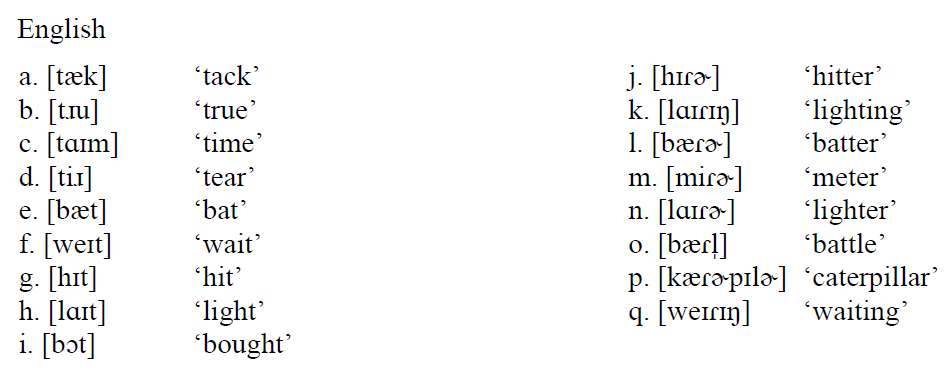
\includegraphics{../images/english_t_flap.png}
\end{figure}

~\\
INSTRUCTOR NOTES: some of the roots alternate (such as 'light'), so we know that we need to analyze the predictable occurrence of [t] vs. [flap]


\vfill
Excellent (3) ~~~ Good (2.2) ~~~ Fair (1.7) ~~~ Poor (0)
\newpage

{\large Question 5}\\

Source: Day 11 Handout, Question 14\\

How does syllabification play a role in the analysis of the phonological relationship between tense and lax high vowels in Quebec French?\\

\begin{figure}[H]
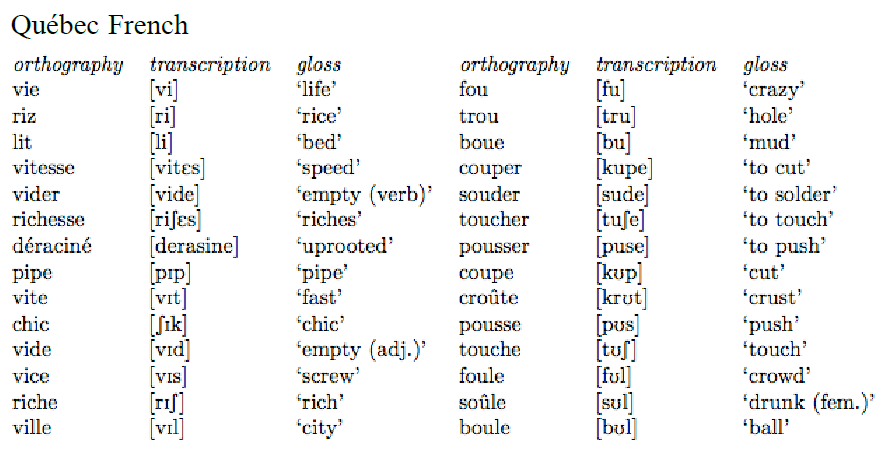
\includegraphics{../images/quebecfrench.png}
\end{figure}

~\\
INSTRUCTOR NOTES: here, syllabification must precede the rest of the analysis; the tense vowels ([i] and [u]) occur in open syllables, while the lax vowels occur in closed syllables -- so e.g. we might have a rule of vowel laxing that says [+high, +syll] --> [-tense] / \_\_ C., with a period to specifically mark the syllable boundary in the context of the rule


\vfill
Excellent (3) ~~~ Good (2.2) ~~~ Fair (1.7) ~~~ Poor (0)
\newpage

{\large Question 6}\\

Source: Quiz 8, Question 6\\

Explain why this is an incorrect statement.\\

Nasal consonants are {[+continuant]} because they lack a central occlusion in the vocal tract.


~\\
INSTRUCTOR NOTES: nasals are [-cont], because air cannot escape through the mouth (there is a central occlusion / blockage)


\vfill
Excellent (3) ~~~ Good (2.2) ~~~ Fair (1.7) ~~~ Poor (0)
\newpage

\begin{center}
\textbf{{\color{red}{\HUGE END OF EXAM}}}\\

\end{center}
\newpage

\begin{center}
\textbf{{\color{blue}{\HUGE START OF EXAM\\}}}

\textbf{{\color{blue}{\HUGE Student ID: empty\\}}}

\textbf{{\color{blue}{\HUGE 4:40 - 5:00 PM\\}}}

\end{center}
\newpage

\begin{center}
\textbf{{\color{blue}{\HUGE START OF EXAM\\}}}

\textbf{{\color{blue}{\HUGE Student ID: 3347\\}}}

\textbf{{\color{blue}{\HUGE 5:00 - 5:20 PM\\}}}

\end{center}
\newpage

{\large Question 1}\\

Source: Quiz 10, Question 3\\

Section 4.2 of chapter 13 in the Peng textbook presented an autosegmental analysis of Mende tone distribution. Explain why the form shown below should NOT be the UR for any morpheme in Mende.\\

\begin{figure}[H]
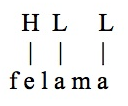
\includegraphics{../images/mende_junction_c.png}
\end{figure}

~\\
INSTRUCTOR NOTES: URs don't have pre-linked tones; the association lines are generated by rules (tone-mapping procedures), AND there's no reason to violate the OCP in the UR of a single morpheme, but this one has two adjacent L tones


\vfill
Excellent (3) ~~~ Good (2.2) ~~~ Fair (1.7) ~~~ Poor (0)
\newpage

{\large Question 2}\\

Source: Final Exam Dataset\\

Explain what the underlying representation of these morphemes would be and why.\\

`invent', `progressive'

\begin{figure}[H]
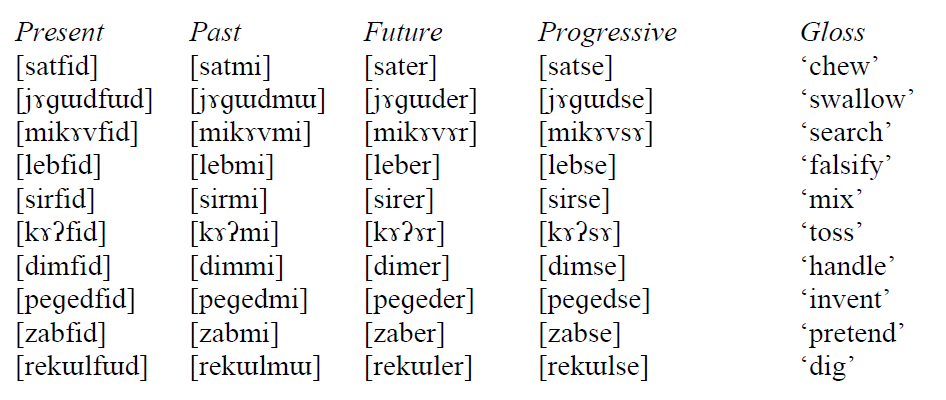
\includegraphics{../images/final_dataset.png}
\end{figure}

~\\
INSTRUCTOR NOTES: For any morpheme that doesn’t alternate, its UR should be the same as its SR.  For the morphemes that alternate, the back-vowel version occurs in the narrower set of contexts (after a back vowel of the same height), so should be the one that we write a rule for. The front-vowel version occurs in the wider / elsewhere set of contexts (after a front vowel and after a back vowel of a different height), so this should be the UR. So in this case, we have the non-alternating root morpheme ‘invent’ /peɡed/ and the alternating suffix morpheme 'progressive' /se/.


\vfill
Excellent (3) ~~~ Good (2.2) ~~~ Fair (1.7) ~~~ Poor (0)
\newpage

{\large Question 3}\\

Source: Quiz 8, Question 3\\

Explain why this featural specification either does or does not match the given sound.\\

{[+consonantal]}, {[+sonorant]}

{[m]}


~\\
INSTRUCTOR NOTES: matches


\vfill
Excellent (3) ~~~ Good (2.2) ~~~ Fair (1.7) ~~~ Poor (0)
\newpage

{\large Question 4}\\

Source: Day 9 Handout, Question 3\\

Explain which morpheme(s) in this dataset alternate and how that helps you do a phonological analysis.\\

\begin{figure}[H]
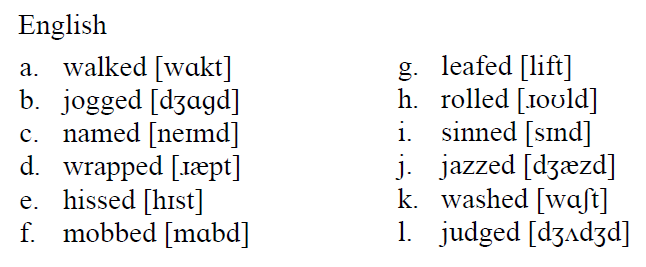
\includegraphics{../images/english_past.png}
\end{figure}

~\\
INSTRUCTOR NOTES: the past tense morpheme alternates, so we know we need to analyze the predictable occurrence of [t] vs. [d]


\vfill
Excellent (3) ~~~ Good (2.2) ~~~ Fair (1.7) ~~~ Poor (0)
\newpage

{\large Question 5}\\

Source: Day 11 Handout, Question 6\\

Explain why this structure either is or is not a correct application of the rule-based approach to syllabification, assuming that both the onset rule and the coda rule apply in this language, and the onset rule comes before the coda rule.\\

\begin{figure}[H]
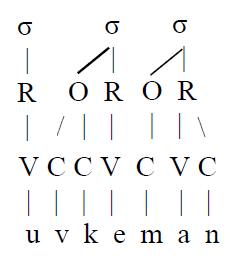
\includegraphics{../images/pengrules_uvkeman_yes.png}
\end{figure}
\begin{figure}[H]
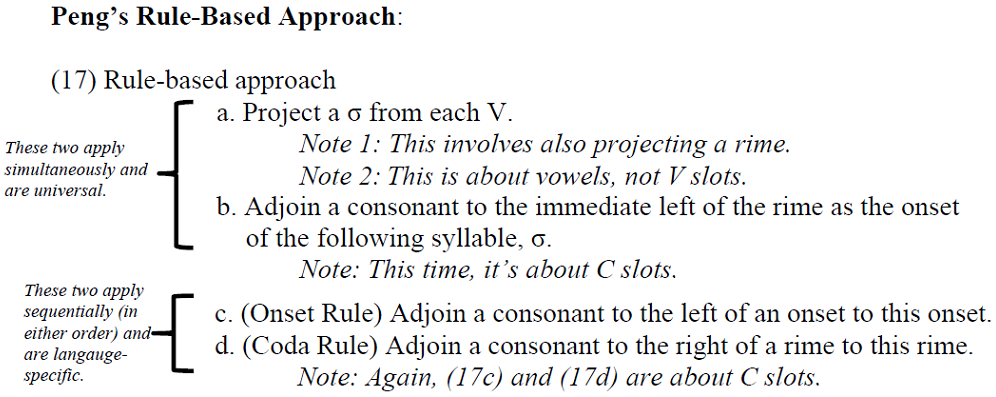
\includegraphics{../images/peng_rules.png}
\end{figure}

~\\
INSTRUCTOR NOTES: yes; the onset rule precedes the coda rule, which puts [v] into the onset (even though that violates sonority), but then we do get the [n] in coda position because it can't go into an onset, and the coda rule does apply


\vfill
Excellent (3) ~~~ Good (2.2) ~~~ Fair (1.7) ~~~ Poor (0)
\newpage

{\large Question 6}\\

Source: Quiz 6, Question 2\\

Explain what you see in the spectrogram that tells you about the properties of the sounds in the pictured word.\\

\begin{figure}[H]
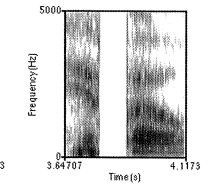
\includegraphics{../images/spectrogram_hippo.png}
\end{figure}

~\\
INSTRUCTOR NOTES: hippo: stop in middle indicated by silence / white space; vowels on either side; V1 has low F1 and high F2 (=high front V) and V2 has higher F1 and lower F2 (=mid to low backer vowel)


\vfill
Excellent (3) ~~~ Good (2.2) ~~~ Fair (1.7) ~~~ Poor (0)
\newpage

\begin{center}
\textbf{{\color{red}{\HUGE END OF EXAM}}}\\

\end{center}
\newpage

\begin{center}
\textbf{{\color{blue}{\HUGE START OF EXAM\\}}}

\textbf{{\color{blue}{\HUGE Student ID: 3420\\}}}

\textbf{{\color{blue}{\HUGE 5:20 - 5:40 PM\\}}}

\end{center}
\newpage

{\large Question 1}\\

Source: Quiz 10, Question 1\\

Section 4.2 of chapter 13 in the Peng textbook presented an autosegmental analysis of Mende tone distribution. Explain why the form shown below should NOT be the UR for any morpheme in Mende.\\

\begin{figure}[H]
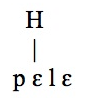
\includegraphics{../images/mende_house_a.png}
\end{figure}

~\\
INSTRUCTOR NOTES: URs don't have pre-linked tones; the association lines are generated by rules (tone-mapping procedures)


\vfill
Excellent (3) ~~~ Good (2.2) ~~~ Fair (1.7) ~~~ Poor (0)
\newpage

{\large Question 2}\\

Source: Final Exam Dataset\\

Explain how you would go about figuring out what to analyse in this dataset.\\

\begin{figure}[H]
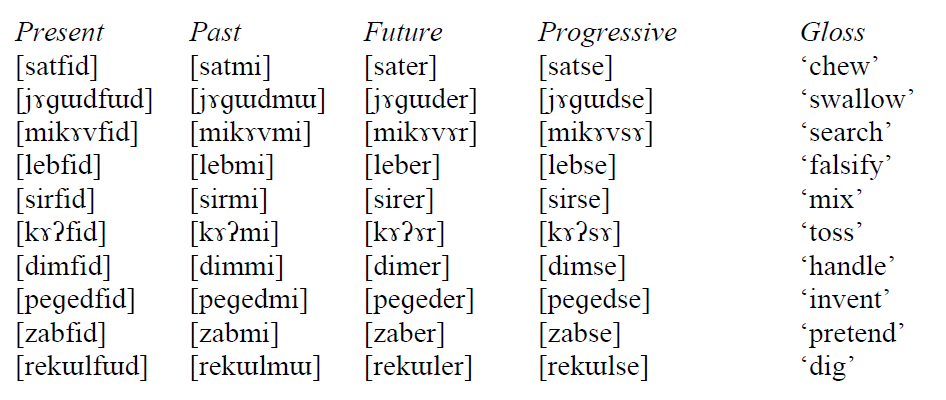
\includegraphics{../images/final_dataset.png}
\end{figure}

~\\
INSTRUCTOR NOTES: The first thing to do is a morphological analysis. There should be morphemes that represent each of the four tenses / aspects (present, past, future, and progressive), and morphemes that represent each root. The morphemes representing the tenses appear as (relatively) consistent forms in the columns; the morphemes representing the roots appear as consistent forms in the rows. Doing this reveals that the final 3 segments in the present forms and the final two segments in the progressive forms are suffixes (there are no zero morphemes, and all components have a one-to-one correspondence). Then we check for alternations. The alternations here are in the suffixes; each of the four suffixes has two forms. There are therefore four alternations, with two allomorphs each. So, what we need to analyze are the alternations in the suffix forms, where we see vowels alternating. Two of the alternations involve [i] and [ɯ], and the other two alternations involve [e] and [ɤ]. In each case, there’s a front vowel and a back vowel, which are otherwise matched for height and rounding, so we can likely generalize across the alternations.


\vfill
Excellent (3) ~~~ Good (2.2) ~~~ Fair (1.7) ~~~ Poor (0)
\newpage

{\large Question 3}\\

Source: Quiz 7, Question 8\\

Based on this data from Lamba, explain why the pair given below either does or does not show that the consonants preceding the morpheme for `with' are NOT responsible for the variation between [-il] and [-el].\\

čit-a \& čit-il-a

\begin{figure}[H]
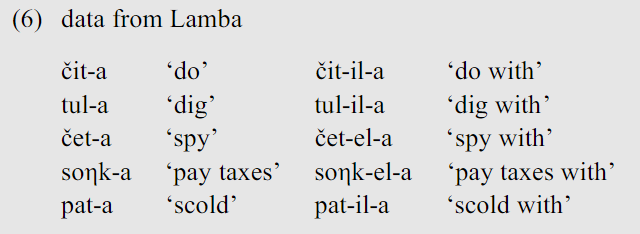
\includegraphics{../images/peng119_lamba.png}
\end{figure}

~\\
INSTRUCTOR NOTES: doesn't show this -- only the [il] form is shown, so we can't judge whether [il] ~ [el] is based on consonants or not


\vfill
Excellent (3) ~~~ Good (2.2) ~~~ Fair (1.7) ~~~ Poor (0)
\newpage

{\large Question 4}\\

Source: Day 11 Handout, Question 10\\

Explain why this structure either is or is not a correct application of the templatic-based approach to syllabification, using the provided template and assuming that syllabification proceeds from left to right.\\

\begin{figure}[H]
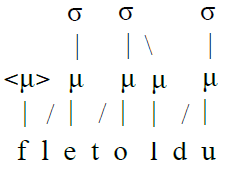
\includegraphics{../images/pengtemplate_fletoldu_no.png}
\end{figure}
\begin{figure}[H]
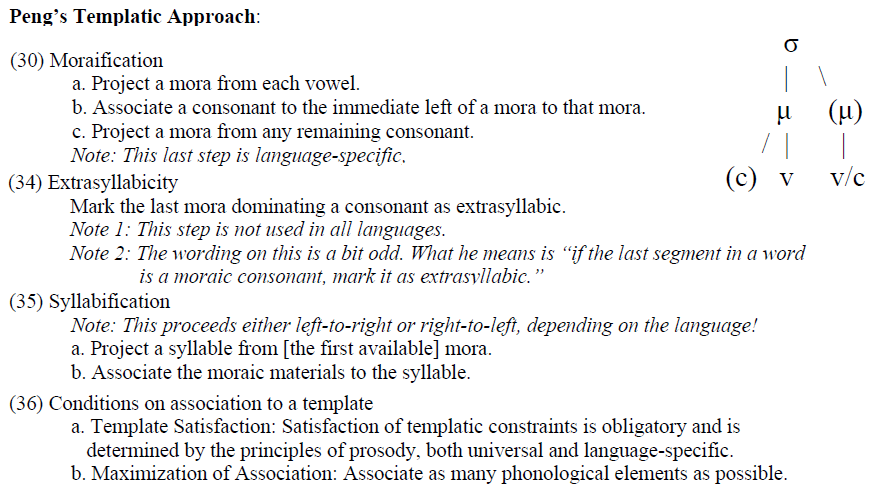
\includegraphics{../images/peng_template_withdiagram.png}
\end{figure}

~\\
INSTRUCTOR NOTES: no -- the initial consonant shouldn't be marked extrasyllabic accoridng to the notes provided


\vfill
Excellent (3) ~~~ Good (2.2) ~~~ Fair (1.7) ~~~ Poor (0)
\newpage

{\large Question 5}\\

Source: Quiz 6, Question 1\\

Explain what you see in the spectrogram that tells you about the properties of the sounds in the pictured word.\\

\begin{figure}[H]
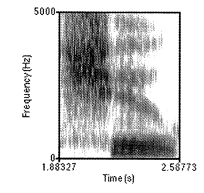
\includegraphics{../images/spectrogram_shoe.png}
\end{figure}

~\\
INSTRUCTOR NOTES: shoe: fricative noise at mid-frequency; no voice bar; vowel formants that suggest low F1 (high V) and low F2 (back V)


\vfill
Excellent (3) ~~~ Good (2.2) ~~~ Fair (1.7) ~~~ Poor (0)
\newpage

{\large Question 6}\\

Source: Quiz 8, Question 3\\

Explain why this featural specification either does or does not match the given sound.\\

{[+consonantal]}, {[-sonorant]}

{[f]}


~\\
INSTRUCTOR NOTES: matches


\vfill
Excellent (3) ~~~ Good (2.2) ~~~ Fair (1.7) ~~~ Poor (0)
\newpage

\begin{center}
\textbf{{\color{red}{\HUGE END OF EXAM}}}\\

\end{center}
\newpage

\end{document}

